\chapter{Results}
\label{ch:Results}

The following chapter will evaluate the results, taking into primary consideration whether interpretable reinforcement learning policies preserve operational performance in power grid topology environments.

\section{Baseline Policies}
\label{sec:baselines}

\begin{table}[H]
\centering
\small
\begin{tabular}{lrrrr}
\toprule
grid & median & mean & min & max \\
\midrule
\multicolumn{5}{l}{\textit{do-nothing (idle)}} \\
bus5    & \textbf{22.04}  & 23.97  & 14.85  & 38.00 \\
bus14   & \textbf{19.96}  & 19.69  & 14.97  & 25.13 \\
bus36-M & \textbf{23.80}  & 23.88  & 21.05  & 26.72 \\
\midrule
\multicolumn{5}{l}{\textit{PPO oracle (teacher)}} \\
bus5    & \textbf{100.00} & 100.00 & 100.00 & 100.00 \\
bus14   & \textbf{68.31}  & 66.85  & 56.51  & 75.66 \\
bus36-M & \textbf{22.56}  & 22.13  & 16.43  & 26.17 \\
\bottomrule
\end{tabular}
\caption{Measured baseline policies.}
\label{tab:baselines}
\end{table}

Observing the do-nothing policies of bus5, bus14, and bus36-M, ranges of 23.15\%, 10.16\%, and 5.67\% are shown. Although this implies that smaller environments showcase a larger spread in their data, this is only across 10 seeds. Such a variation in survival rate immediately denotes a significant difference in difficulty based on seed selection. From the baseline policies itself, we observe that the seed selection plays a crucial role in how well a policy generalises and converges to a strong solution. Additionally, it is clear that the survival rate drops substantially as the complexity of the environment increases, as showcased by the median and mean values. There exists greater variance in the range for the teacher oracle for both bus14 and bus36-M, with the only grid environment showcasing perfect learning being bus5, which is able to attain 100\% survival rate across all ten seeds tested. Initially, it seems as though the do-nothing policy is stronger than the PPO teacher oracle, but this is once again attributed to how much variety each seed introduces into the testing protocol, causing these mismatches. This is not a drawback of the protocol itself, but rather a fundamental aspect regarding the functionality of the RL2Grid benchmark and its heavy reliance on seed selection for obtaining high-quality output data due to less demanding situations that the input data may potentially provide.

\section{All Methods}

The most valuable analysis derives from the bus14 grid, with the other two grids in Table \ref{sec:master} not showcasing meaningful data. Observing bus5, we see that this environment is extremely saturated due to low complexity. This is reflected by the interpretable models and the PPO teacher oracles being able to successfully learn the environment extremely well. Not only does the teacher oracle reaches a 100\% survival rate, but also the original DTPO algorithm and our improved GDTPO algorithm do so as well. At first glance, it seems as though VIPER, DAgger, and one-shot distillation are extremely poor at distilling the policy from the teacher oracle; however, the mean being significantly higher than the median signifies that the seed selection plays a crucial role. Within two individual seeds, VIPER is able to hit 100\% survival rate, and the highest survival rate achieved by DAgger and one-shot distillation was 81.17\% and 81.10\% respectively.

\label{sec:master}

\begin{table}[H]
\centering
\footnotesize
\setlength{\tabcolsep}{4pt}
\renewcommand{\arraystretch}{1.15}
\begin{tabular}{lccc}
\toprule
\textbf{method} & \textbf{bus5} ($n{=}5$) & \textbf{bus14} ($n{=}10$) & \textbf{bus36-M} ($n{=}5$) \\
\midrule
\textbf{do-nothing} & \textbf{22.04} / 23.97 & \textbf{19.96} / 19.69 & \textbf{23.80} / 23.88 \\
\textbf{PPO oracle (teacher)} & \textbf{100.00} / 100.00 & \textbf{68.31} / 66.85 & \textbf{22.56} / 22.13 \\
\midrule
DTPO (Alg.~\ref{alg:dtpo})
  & \rcell{100.00 / 89.93}{}
  & \rcell{29.62 / 35.39}{}
  & \rcell{23.80 / 23.88}{} \\
\textbf{GDTPO (Alg.~\ref{alg:gdtpo})}
  & \rcell{\textbf{100.00} / 84.93}{}
  & \rcell{\textbf{51.20} / 52.42}{}
  & \rcell{\textbf{23.80} / 23.68}{} \\
\midrule
VIPER
  & \rcell{31.62 / 55.52}{}
  & \rcell{28.76 / 33.84}{}
  & \rcell{13.40 / 15.55}{} \\
DAgger (tree student)
  & \rcell{6.17 / 30.83}{}
  & \rcell{13.52 / 20.72}{}
  & \rcell{21.05 / 18.55}{} \\
one-shot distillation
  & \rcell{17.14 / 28.55}{}
  & \rcell{33.44 / 31.34}{}
  & \rcell{21.05 / 19.77}{}\\

\bottomrule
\end{tabular}
\caption{Final results across the three grids, with a 16 leaf budget. Each cell reports the median followed by the mean.}
\label{tab:master}
\end{table}

Since VIPER fits a decision tree classifier on hard labels, vital information might be disregarded, causing a drop in survival rate within this domain. Moreover, DAgger collates states visited by the student tree, which may be full of observations that the teacher oracle has never seen before, once again causing this drop in survival rate.

On the other hand, all DTPO-related methods for bus36-M seem to reproduce the do-nothing policy almost exactly. Interestingly, the PPO oracle, although supposed to be stronger, actually showcases a slightly weaker survival rate, with a mean delta of -1.76\%. This could be attributed to the PPO teacher oracle having substantially more actions to choose from; if the probability vectors of the actions possible are similar, an unintended action may be taken that causes cascading effects on the grid. We observe that the DTPO-related methods essentially output the do-nothing policy.  

This means that two of the three grids tested have very minimal statistics to report; bus5 is too easy to learn, and bus36-M leads all methods to essentially converge towards the same behaviour of the do-nothing policy, where no action takes place. Therefore, for the rest of the results, bus14 shall stay as the primary focus. Initial tests on 5 seeds showcased the oversaturated and undersaturated behaviour of policies on bus5 and bus36-M respectively. Due to their uninformative nature, computational resources were reallocated to bus14, where 10 seeds were used.

\begin{table}[H]
\centering
\small
\begin{tabular}{lrrrrrr}
\toprule
bus14, 16 leaves, $n=10$ & med & mean & $\Delta$ (med) & $\Delta$ (mean) & signs & \% teacher \\
\midrule
DTPO & 29.62 & 35.39 & $+$9.75 & $+$15.70 & 10/10 & 41.2\% / 53.8\% \\
\textbf{GDTPO} & \textbf{51.20} & \textbf{52.42} & \textbf{$+$32.70} & \textbf{$+$32.73} & 10/10 & \textbf{85.3\%} / \textbf{77.8\%} \\
\bottomrule
\end{tabular}
\caption{End-to-end comparison of two complete configurations of the DTPO algorithm as published and our improvement, GDTPO, on bus14.}
\label{tab:endtoend}
\end{table}

Observing the bus14 algorithm on 16 leaves, we can compare the original DTPO algorithm to our improved GDTPO algorithm (also referred to as \texttt{dtpo-full}); both methods are able to surpass the do-nothing baseline on all ten seeds. The GDTPO algorithm also improves substantially on the original DTPO algorithm for this domain, with the median rising from 29.62\% to 51.20\%. Comparing the medians, this value does not seem impressive at first glance. However, in comparison with the teacher oracle, we see promising results in GDTPO, showcasing significant recovery of the teacher oracle in comparison with DTPO. We can successfully conclude that our modified algorithm is able to \textbf{recover on average 77.8\% of its teacher}.

\section{Ablation Study}

\label{sec:ablation}

Since we wish to understand in detail the contribution of each specific component in the newly devised approach, an ablation study has been conducted to help understand where exactly the improvement within the model comes from. 

\begin{table}[H]
\centering
\footnotesize
\setlength{\tabcolsep}{6pt}
\renewcommand{\arraystretch}{1.15}
\begin{tabular}{lcccc}
\toprule
\textbf{DTPO method} & \textbf{warm start} & \textbf{gate} & \textbf{replay} & \textbf{refit} \\
\midrule
\texttt{dtpo} \emph{(DTPO)}   & $\times$     & $\times$     & $\times$          & $\times$          \\
\texttt{dtpo-ws}              & \checkmark   & $\times$     & $\times$          & $\times$          \\
\texttt{dtpo-scratchgate}     & $\times$     & \checkmark   & $\times$          & $\times$          \\
\texttt{dtpo-gate-K1}         & \checkmark   & \checkmark   & $\times$          & $\times$          \\
\texttt{dtpo-replay}          & \checkmark   & $\times$     & \checkmark & \checkmark \\
\texttt{dtpo-gate}            & \checkmark   & \checkmark   & $\times$          & \checkmark \\
\texttt{dtpo-scratchfull}     & $\times$     & \checkmark   & \checkmark & \checkmark \\
\textbf{\texttt{dtpo-full}} \emph{(GDTPO)} & \checkmark & \checkmark & \checkmark & \checkmark \\
\bottomrule
\end{tabular}
\caption[Configuration of every DTPO variation]{Configuration of DTPO variants tested across the three grids.}
\label{tab:dtpo-configs}
\end{table}

The eleven methods listed in Table~\ref{tab:headline} correspond to specific variations tested. As aforementioned, \textit{dtpo-full} and \textit{dtpo} refer to the GDTPO and DTPO algorithms as published, respectively. The methods \textit{viper} and \textit{daggertree} are the decision-tree students produced by VIPER and by DAgger with a tree student, and \textit{distill} collects demonstrations from the PPO oracle once and fits a single tree to them. To attribute the effect of each component of GDTPO, the configurations of Table~\ref{tab:dtpo-configs} differ from one another by a single flag, some via an additive approach to DTPO, and others through a subtractive approach from GDTPO, so that any paired difference is attributable to that improvement alone.

Decoupled structure refitting is not removed from the full configuration. Doing so would lead to the structure being regrown every iteration while the buffer still holds grid state data collected under previously disregarded tree structures. As a topology action changes the grid state from which all later observations are drawn, these states are those that the new structure would rarely visit. Keeping the buffer would reintroduce instability, as the tree would spend the leaf budget partitioning regions not occupied by the new structure. Refitting is instead isolated between \textit{dtpo-gate} and \textit{dtpo-gate-K1}, which differ only in the refit period. The ablation study data is shown in Table~\ref{tab:headline}.

\begin{table}[H]
\centering
\footnotesize
\setlength{\tabcolsep}{4pt}
\begin{tabular}{lrrrrrrrr}
\toprule
& & \multicolumn{2}{c}{survival} & \multicolumn{2}{c}{$\Delta$ vs idle}
& & \multicolumn{2}{c}{\% of teacher} \\
\cmidrule(lr){3-4}\cmidrule(lr){5-6}\cmidrule(lr){8-9}
method & $n$ & med & mean & med & mean & signs & med & mean \\
\midrule
\texttt{dtpo-full} \emph{(GDTPO)} & 10 & 51.20 & \textbf{52.42} & $+$32.70 & \textbf{$+$32.73} & \textbf{10/10} & \textbf{85.3\%} & \textbf{77.8\%} \\
\texttt{dtpo-replay} & 10 & 55.44 & 51.43 & \textbf{$+$35.32} & $+$31.74 & 10/10 & 82.6\% & 77.0\% \\
\texttt{dtpo-scratchgate} & 10 & 49.69 & 50.60 & $+$26.11 & $+$30.91 & 10/10 & 76.0\% & 75.7\% \\
\texttt{dtpo-gate} & 10 & 48.53 & 46.43 & $+$26.68 & $+$26.74 & 10/10 & 66.7\% & 69.6\% \\
\texttt{dtpo-ws} & 10 & \textbf{55.50} & 48.85 & $+$32.09 & $+$29.16 & 10/10 & 77.5\% & 73.4\% \\
\texttt{dtpo-gate-K1} & 10 & 43.18 & 39.79 & $+$22.11 & $+$20.10 & 9/10 & 66.8\% & 59.5\% \\
\texttt{distill} & 10 & 33.44 & 31.34 & $+$13.11 & $+$11.65 & 7/10 & 50.0\% & 47.4\% \\
\texttt{dtpo} & 10 & 29.62 & 35.39 & $+$9.75 & $+$15.70 & 10/10 & 41.2\% & 53.8\% \\
\texttt{viper} & 10 & 28.76 & 33.84 & $+$5.34 & $+$14.15 & 6/10 & 39.3\% & 51.4\% \\
\texttt{dtpo-scratchfull} & 10 & 22.85 & 23.60 & $+$2.30 & $+$3.91 & 8/10 & 37.1\% & 35.5\% \\
\texttt{daggertree} & 10 & 13.52 & 20.72 & $-$4.91 & $+$1.03 & 4/10 & 21.2\% & 32.9\% \\
\bottomrule
\end{tabular}
\caption{Bus14 at 16 leaves, ordered by mean of the survival rate. Differences and ratios are computed within a seed and aggregated
afterwards; \emph{signs} counts seeds on which the configuration exceeds do-nothing.
\% of teacher is the median and mean of the per-seed ratio to the PPO oracle.
All eleven configurations have the full seed set 100--109.}
\label{tab:headline}
\end{table}

We see that both the warm start and the gate mechanism play a major role in boosting the original DTPO's average survival rate, from 35.39\% to 48.85\% and 50.60\% respectively. When the other three modifications are present, introducing a teacher oracle to warm start the student policy improves on all ten seeds. If DTPO is observed to incorporate these other modifications without including a teacher oracle and training from a singular leaf from scratch, this degrades the policy in comparison with its original DTPO algorithm. However, this does not invalidate the ablation study - we do not see the best results unless all four modifications are present, as showcased by the other methods such as \textit{dtpo-gate} and \textit{dtpo-scratchgate}, where we do see improvements in the survival rate and the percentage of the teacher oracle recovered, with these values observed at 69.6\% and 75.7\% respectively.

Our full configuration is not the best of the variants run with regards to the median, with the original DTPO algorithm warm started with a PPO teacher oracle showcasing the highest median survival rate at 55.50\%. Nonetheless, the GDTPO algorithm with all four improvements showcases the strongest recovery of the teacher oracle with regards to the mean and median, as well as the highest mean survival rate. This highlights that the survival gate is not meant to make the final policy better, but rather prevents a policy that is already good from being replaced by one that is worse, improving stability as hypothesised. A higher mean value showcases this improvement in stability.
 
Thus, warm starting from a teacher oracle serves as the most significant modification to DTPO, showcasing how important the teacher oracle is to training a student policy. This point is further emphasised across all results collated, due to the fact that none of the results are able to surpass the baseline set by the teacher oracle. 

Within the scope of this study, we identify that none of the configurations surpassed the teacher oracle. Thus, we hypothesise that results in this field of reinforcement learning and power grid operations will continue to be limited by the strength of the teacher oracle, and future work must aim towards bettering this area.

\section{Leaf Budget}

\begin{table}[H]
\centering
\small
\begin{tabular}{lrrrr}
\toprule
bus14, median / mean & 8 leaves & 16 leaves & 32 leaves & 64 leaves \\
\midrule
\texttt{dtpo-full} & 47.20 / 39.30 & 51.20 / 52.42 & 27.22 / 28.18 & 10.03 / 20.28 \\
\texttt{distill} & 46.19 / 40.63 & 33.44 / 31.34 & 8.27 / 16.09 & 5.84 / 14.15 \\
\texttt{viper} & 38.43 / 41.72 & 28.76 / 33.84 & 38.12 / 32.16 & 17.16 / 21.71 \\
\texttt{daggertree} & 12.69 / 17.81 & 13.52 / 20.72 & 32.98 / 36.90 & 22.67 / 27.95 \\
\midrule
\textit{do-nothing} & \multicolumn{4}{c}{\textit{19.96 / 19.69}} \\
\bottomrule
\end{tabular}
\caption{Survival rates on bus14 on differing leaf budgets. Cell sizes are $n=10$ at 16 leaves and $n=5$ elsewhere.}
\label{tab:frontier}
\end{table}

Since we aim to understand the interpretability aspect, we also tested developing decision trees with differing leaf budgets in powers of 2, from 8 to 64. 8 was chosen as the lower bound as viable policies were not produced below this, whereas there was no valid reason to have more than 64 leaves, given that we were limiting our work within difficulty 0, where the maximum number of actions is 50. 

All four policies used all of the allocated leaf budget when creating their tree. When a tree has $x$ leaves, the minimum depth of the tree is $\lceil\log_2 x\rceil$. For 16-leaf trees, although the minimum depth is 4, the depth of the trees varied, with the GDTPO algorithm producing trees of median depth 6, while other methods such as VIPER and DAgger produce trees with a median depth of 8. Overall, initial observations support an association between shallower trees and a comparatively better survival rate. However, this should not be taken as the final overarching conclusion, as within GDTPO itself, the depth varies depending on the run, changing between 5 and 9 (inclusive). We aim to clarify that the optimisation of depth, or optimisation strategies such as pruning, were not prioritised for consistency purposes. For this reason, and due to the fact that the argmax probability of action is taken from the probability vector, sometimes both leaves of a node showcase the exact same action. In general, the best survival rate is observed when the leaf budget is set to 16 leaves, which is why a large portion of the experimentation was fixed at this value, and then 10 runs were conducted for the previous ablation study. 

Through the inclusion of a teacher oracle, however, the benefit of having an initial policy to distil from is prominent, as the policies where warm-starting exists have more balanced structures, whereas policies trained from scratch have greater depth and are forced to discover the policy rather than have a foundation on which to build upon. 

Another observation is how unstable the survival rate becomes as the number of leaves is increased. This is observed within the listing of every run for GDTPO on bus14, as shown in Table~\ref{tab:frontier-seeds} where the run with the lowest survival rate outputs 6.05\%, whereas one seed is able to output 58.22\%. Once again, this showcases the importance of seed selection in attaining a good survival rate. We cannot completely confirm that the new GDTPO method is able to outperform its counterparts at every leaf budget, as it degrades at 32 and 64 leaves within bus14. This hints towards the importance of further fine-tuning and optimisation in order to attain a high survival rate and obtain a strong interpretable policy.

\begin{table}[H]
\centering
\small
\begin{tabular}{ll}
\toprule
\texttt{dtpo-full}, bus14 & per-seed report survival, sorted \\
\midrule
8 leaves  & 56.48\; 49.31\; 47.20\; 21.80\; 21.69 \\
16 leaves & 74.48\; 67.43\; 66.54\; 63.53\; 53.57\; 48.82\; 45.21\; 43.01\; 40.46\; 21.14 \\
32 leaves & 45.93\; 41.73\; 27.22\; 13.61\; 12.43 \\
64 leaves & 58.22\; 18.81\; 10.03\; 8.27\; 6.05 \\
\bottomrule
\end{tabular}
\caption{Every run behind the \texttt{dtpo-full} row of
Table~\ref{tab:frontier}. Medians conceal how unstable the larger budgets are.}
\label{tab:frontier-seeds}
\end{table}

\begin{figure}[H]
\centering
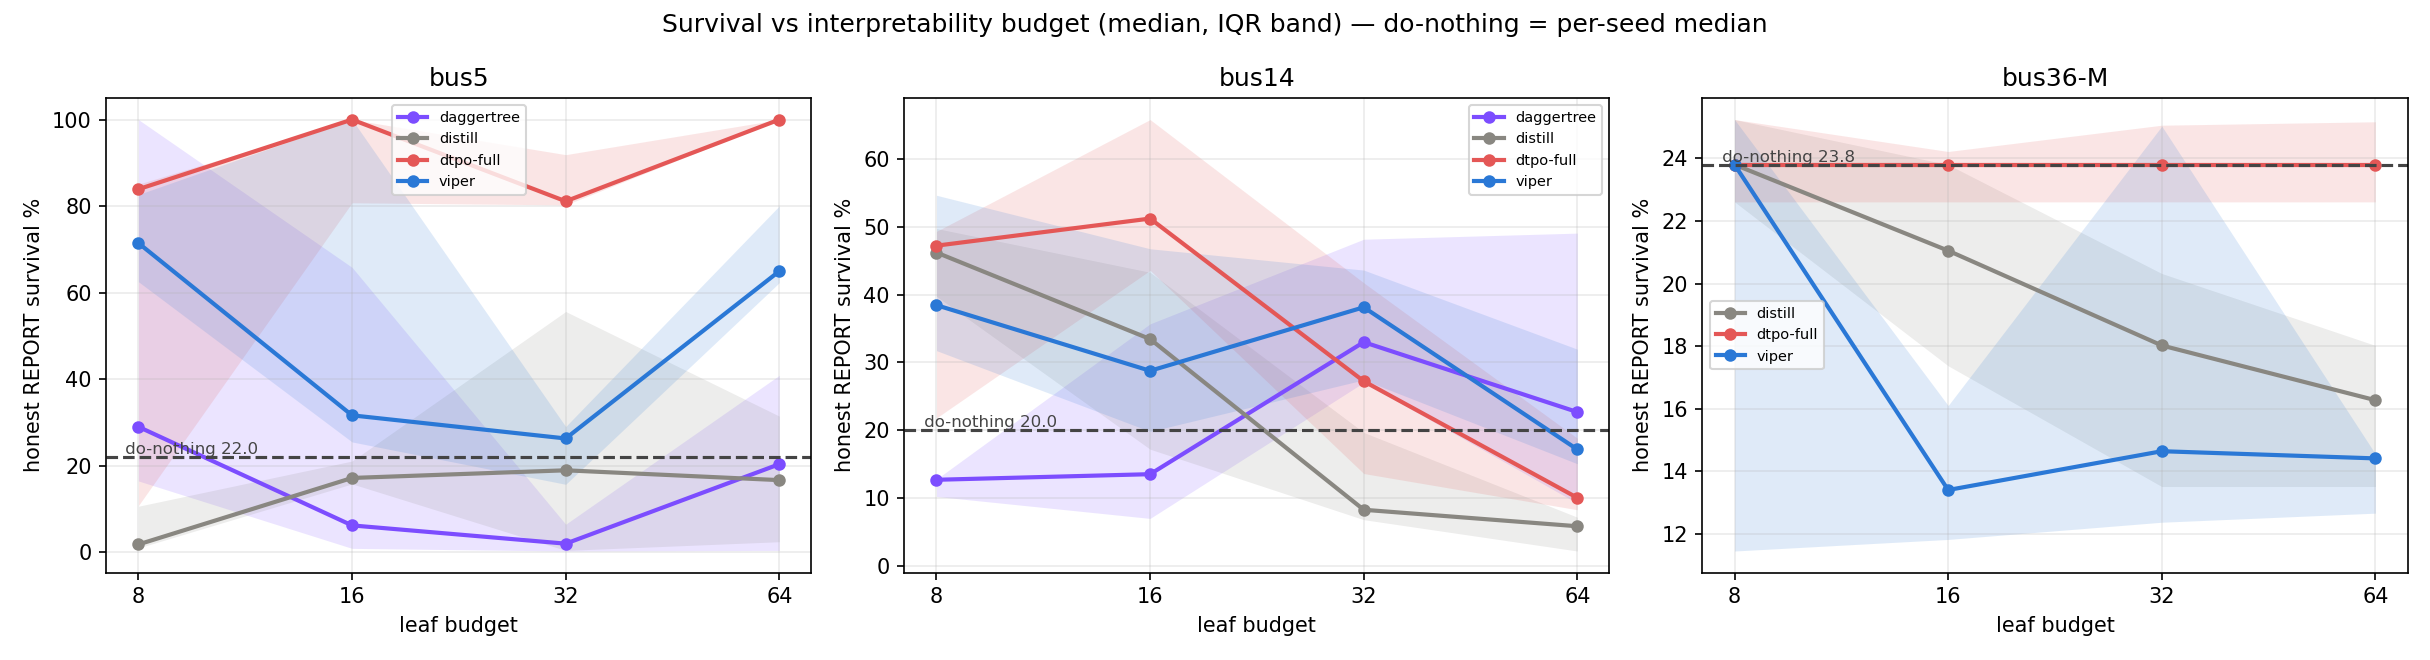
\includegraphics[width=\textwidth]{figures/frontier.png}
\caption{Median report survival against leaf budget, per method and grid, with
the interquartile band. The trade-off inverts on bus14: 8--16 leaves dominates
64.}
\label{fig:frontier}
\end{figure}

A plausible explanation as to why GDTPO performs better at 16 leaves, whereas VIPER and DAgger perform better with more leaves is that more leaves provides methods like VIPER and DAgger a greater breadth to reproduce the actions of the teacher. On the other hand, policies like GDTPO and one-shot distillation differ by actively optimising within the environment itself, instead of fully relying on the teacher oracle (albeit they do utilise it for initial policy establishment). Regardless, one thing that can be corroborated once again is the importance of seed selection as well as the requirement for more tests to obtain more data for quality assurance and ensuring consistency.

\begin{figure}[H]
\centering
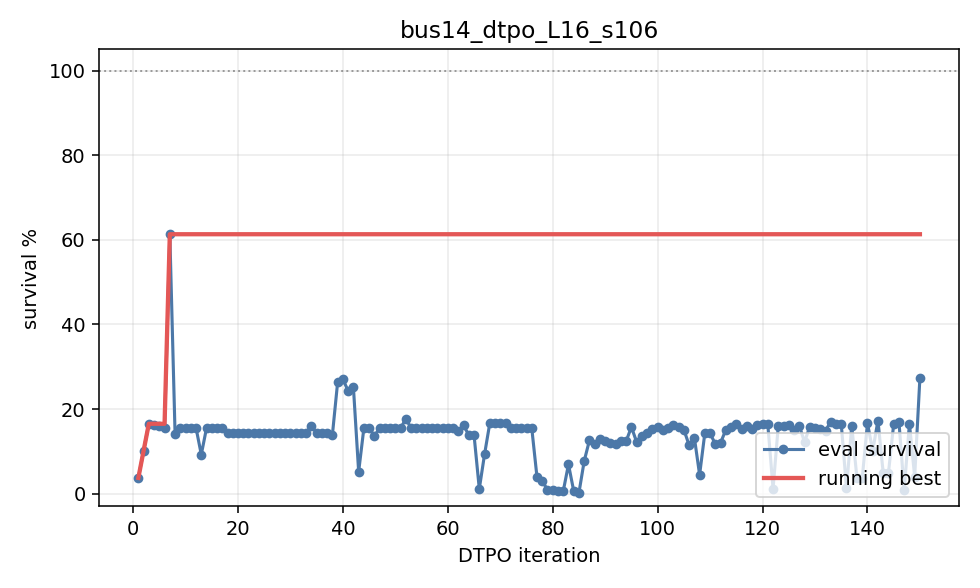
\includegraphics[width=0.85\textwidth]{figures/dtpo_l16_s106.png}
\caption{A single training run (\texttt{bus14\_dtpo\_L16\_s106}):
per-evaluation deployed survival and running best across the 150 iterations.}
\label{fig:curve}
\end{figure}

\begin{figure}[H]
\centering
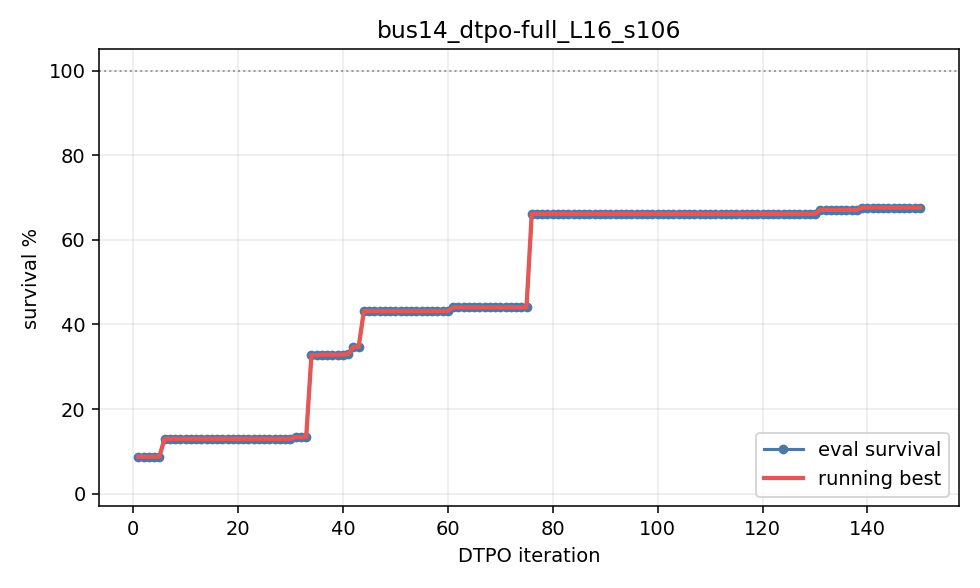
\includegraphics[width=0.85\textwidth]{figures/curve_dtpo-full_s106.png}
\caption{A single training run (\texttt{bus14\_dtpo-full\_L16\_s106}):
per-evaluation deployed survival and running best across the 150 iterations.}
\label{fig:curve2}
\end{figure}

Without the presence of a survival gate, training is erratic and unstable, especially when interpretable policies are being developed. This is seen within black-box models as well, with small improvements as the number of training timesteps and iterations increases, but this is extremely time-consuming and resource-demanding. The inclusion of a survival gate does not necessarily help improve the policy, but rather ensures that a new policy is always at least better than or equal to the previous policy it replaces, and therefore serves as a positive addition to the model for this domain.

% This is showcased in \ref{fig:gate-filter}. 

Although all results report the survival rate, as it is the primary metric that we have based our evaluation on, it should be noted that the cost of evaluation of every policy is considerable. For all policies except one-shot distillation from the PPO oracle, each policy is run for 150 iterations, each including 10,000 timesteps. This gives a combined total of 1.5 million timesteps. On the other hand, the one-shot distillation policy only runs for 20,000 environmental timesteps, with no active reinforcement learning taking place. 

\section{Policy Visualisation}

\begin{figure}[H]
\centering
\includesvg[width=\textwidth,inkscapelatex=false]{figures/tree_warmstarted_s106}
\caption{A warm-started 16-leaf policy on bus14
(\texttt{dtpo-full}, seed 106).}
\label{fig:tree-warm}
\end{figure}

\begin{figure}[H]
\centering
\includesvg[width=\textwidth,inkscapelatex=false]{figures/tree_fromscratch_s100}
\caption{The same budget trained from scratch
(\texttt{dtpo-scratchfull}, seed 100), for comparison with
Figure~\ref{fig:tree-warm}.}
\label{fig:tree-scratch}
\end{figure}

% \begin{figure}[H]
% \centering
% 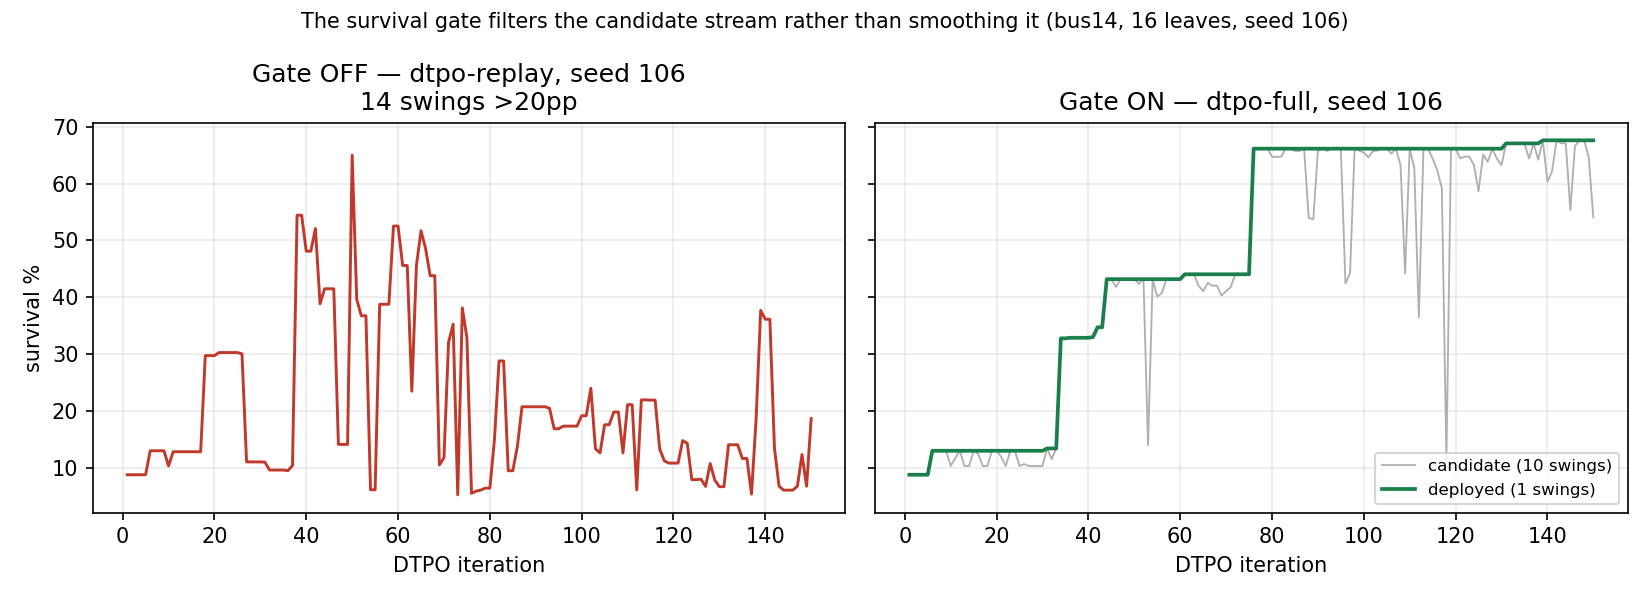
\includegraphics[width=\textwidth]{figures/gate_before_after_s106.png}
% \caption{The survival gate as a filter (bus14, 16 leaves, seed
% 106).}
% \label{fig:gate-filter}
% \end{figure}


Within the visualisation of the trees, each node consists of the observation attribute and a comparative with a value, and its leaves consist of two variables, namely the action as well as its respective $p$, the average probability assigned to this action by the stochastic policy. As the tree is fit as a regressor onto a normalised target over distributed actions, the action with the largest $p$ is finally chosen. Although the policy during training is stochastic, the deployed policy through the interpretable decision tree is ultimately deterministic. The closer the value of $p$ is to 1.00, the more likely the policy preferred this action, and vice versa; the closer the value of $p$ is to 0.02 (since there are 50 actions possible in total, making 0.02 the uniform value), the more equally probable each possible action was. 

This does not fully indicate that some trees are more confident than others. Within the strongest interpretable policies trained, we see that some leaves showcase $p$ up to 0.99, showcasing high confidence, whereas other leaves may have a $p$ as low as 0.04. By this understanding, the results of bus36-M may be construed to be anomalous, since some seeds contain nodes with both child leaves showcasing the action 0 of ``do-nothing'' with $p = 1.00$, essentially reverting to exactly the same policy as do-nothing. This could be due to two reasons. The first is that the policies truly converge towards the do-nothing action, as the teacher policy itself tends to idle and rarely produces other actions that have an impact on the environment. But since the policies of DTPO configurations trained from scratch tend to return the exact same values as that of the do-nothing policies, this suggests a discrepancy between the actions suggested by the decision tree from its policy learning, and the action space itself. We observe that some seeds within bus36-M, such as seeds 101 and 103, do showcase other actions in their leaves, yet still output the same policy as do-nothing. These actions specifically are actions that allow for more than one substation to be changed within the same timestep. Thus, this suggests that the environment is unable to accept actions that impact more than one substation simultaneously, causing a revert to the default do-nothing action. This is another reason why the bus36-M results are not prioritised, and bus14 and bus5 are preferred in that order, as the anomalous data of bus36-M can be attributed to the inherent action space file being inconsistent with the environment itself. This will require further testing to confirm this hypothesis, and shall be detailed in future work. 

The value of $p$ has been intentionally included such that human-operators utilising these decision trees to take decisions will be able to understand how confident the policy is in choosing a certain action for a leaf. 

\section{Fidelity}

Through fidelity, we aim to measure whether a distilled policy is able to reproduce the actions of its teacher oracle. Each policy is measured on two state distributions: those visited by the oracle, and those visited by the tree itself. Both use the same environment, evaluation, and start, only differing in the action executed, thereby showcasing the divergence in trajectories. The former questions whether the tree is able to learn how the teacher operates in its trajectory, whereas the latter questions whether the actions suggested agree even when the trajectory of the environment changes due to the actions of the tree. Measurements are done over ten episodes per run, and shown in Table~\ref{tab:fidelity}. We observe that every configuration loses fidelity moving from the oracle-visited states to the tree-visited states. This loss is unsurprisingly smallest for the imitation methods like one-shot distillation (\textit{distill}) and DAgger, where the average weighted fidelity falls from 0.799 to 0.620 and 0.746 to 0.527 respectively.

\begin{table}[H]
\centering
\footnotesize
\setlength{\tabcolsep}{4pt}
\begin{tabular}{lrrrrrrrrr}
\toprule
& & \multicolumn{4}{c}{on oracle-visited states} & \multicolumn{4}{c}{on tree-visited states} \\
\cmidrule(lr){3-6}\cmidrule(lr){7-10}
& & \multicolumn{2}{c}{fidelity} & \multicolumn{2}{c}{weighted} &
    \multicolumn{2}{c}{fidelity} & \multicolumn{2}{c}{weighted} \\
\cmidrule(lr){3-4}\cmidrule(lr){5-6}\cmidrule(lr){7-8}\cmidrule(lr){9-10}
method & $n$ & med & mean & med & mean & med & mean & med & mean \\
\midrule
\texttt{distill} & 10 & 0.606 & 0.612 & 0.801 & 0.799 & 0.497 & 0.483 & 0.659 & 0.620 \\
\texttt{daggertree} & 10 & 0.557 & 0.556 & 0.747 & 0.746 & 0.470 & 0.398 & 0.648 & 0.527 \\
\texttt{viper} & 10 & 0.437 & 0.442 & 0.589 & 0.564 & 0.382 & 0.371 & 0.494 & 0.481 \\
\texttt{dtpo-gate-K1} & 10 & 0.441 & 0.445 & 0.506 & 0.500 & 0.134 & 0.153 & 0.200 & 0.180 \\
\texttt{dtpo-gate} & 10 & 0.432 & 0.435 & 0.502 & 0.512 & 0.163 & 0.199 & 0.238 & 0.247 \\
\texttt{dtpo-full} \emph{(GDTPO)} & 10 & 0.420 & 0.415 & 0.501 & 0.496 & 0.213 & 0.219 & 0.245 & 0.261 \\
\texttt{dtpo-ws} & 10 & 0.385 & 0.395 & 0.412 & 0.452 & 0.177 & 0.182 & 0.180 & 0.196 \\
\texttt{dtpo-replay} & 10 & 0.381 & 0.370 & 0.390 & 0.393 & 0.184 & 0.180 & 0.234 & 0.217 \\
\midrule
\texttt{dtpo-scratchfull}$^{\dagger}$ & 10 & 0.207 & 0.182 & 0.117 & 0.110 & 0.002 & 0.018 & 0.001 & 0.012 \\
\texttt{dtpo-scratchgate}$^{\dagger}$ & 10 & 0.134 & 0.136 & 0.101 & 0.116 & 0.042 & 0.104 & 0.032 & 0.137 \\
\texttt{dtpo}$^{\dagger}$ & 10 & 0.063 & 0.103 & 0.038 & 0.059 & 0.007 & 0.028 & 0.009 & 0.030 \\
\bottomrule
\end{tabular}
\caption[Tree--oracle fidelity on bus14]{%
\textbf{Fidelity between each distilled tree and the PPO teacher} on bus14 at a
sixteen-leaf budget, over ten seeds. Rows are ordered by weighted fidelity on oracle-visited states. Configurations marked $\dagger$ were trained without a teacher.}
\label{tab:fidelity}
\end{table}

As we are aiming to optimise the survival rate, the inclusion of a teacher oracle via the warm start mechanism does improve the fidelity, but invariably do not reach the same fidelity as the pure imitation methods. As anticipated, the three counterparts which were trained without a teacher showcase the lowest fidelity, with the original DTPO method possessing a mean weighted fidelity of 0.059. This confirms that the presence of the teacher oracle during training does have an impact on the similarity of the policies between the teacher and the student.

Compared against the survival rate results in Table~\ref{tab:headline}, we see there is no clear indication that fidelity and survival rate go hand in hand. Configurations like \texttt{dtpo-scratchgate} have one of the lowest fidelity rates, as it was not trained with the teacher oracle, but attains an average survival rate higher than one-shot distillation, which attained the highest fidelity values across the eleven configurations on bus14. 

A limitation of this fidelity study is that we only compare the behaviour of our configurations on a specific PPO oracle teacher checkpoint. Furthermore, survival and fidelity are heavily dependent on the trajectory of the environment based on the actions taken; since the fidelity is calculated as a ratio measuring the similarity between the actions of the teacher and the student, the fidelity value can immediately derail, depending on how earlier a discrepancy occurs between the two. 

\section{Discussion}


Several aspects of this research were found to be difficult to navigate, and all factors will be discussed here in detail as the project's limitations and threats to validity.

\textbf{Seed selection.} Since each seed of the environment selects its own set of chronics, where each series of chronics differs in difficulty, it is extremely challenging to produce reliable and stable checkpoints across all seeds. This was the reason why the chronics evaluated upon were fixed; even though the consistency and stability can be improved through a greater number of tests, the CPU resources required would be extensive, which is why our runs were limited to a maximum of ten per method tested.

\textbf{Chronics.} Additionally, our choice of chronics may have also swayed the selection and choice of the decision trees. Due to both resource and time constraints, all the remaining chronics were not used for validation and testing, and this could be changed within the methodology for a better understanding of how the decision trees would perform in more environment scenarios.

\textbf{Teacher oracle.} Checkpoints trained by the benchmark do not store the observation normalisation statistics under which the policies are trained, and so it is difficult to evaluate or reproduce the policy unless the environment and agent seed are known. To ensure stability of the teacher oracle, we therefore obtained the final checkpoints of the PPO teacher oracle of bus5 and bus14 directly from the authors of RL2Grid, which saved significant training time. The training of the bus36-M oracle took over three continuous weeks on a local machine. Initial testing within the interim report also focused on identifying strong DQN oracles, but these were disregarded due to their instability and weakness in comparison with their PPO counterparts. Therefore, further testing is required to test the methods and complete an ablation study on multiple teacher oracles, rather than only one. Methods like VIPER are also primarily designed to distil a complex deep neural network policy, making DQN oracles the better choice. However, due to the availability and strength of PPO oracles, the implementation of VIPER was therefore adapted to not only fit the requirements of RL2Grid, but also obtain the action-probability gap between the top two actions as a replacement for the lack of Q-values in the stochastic policy.

\textbf{Training cost.} The cost of training and evaluation played a crucial role in the design of these experiments. Given the computational resources, the number of iterations can also be increased further, to see the impact on training and testing and observe at which point the survival rate saturates and plateaus in its growth. Given the size and complexity of the environment, and time taken for training any policy, the number of iterations had to be limited to 150. It remains completely possible that the published algorithms as well as our improved algorithm showcase improvement on all grid types as the opportunity for compute increases. Furthermore, solely looking at the results elaborated upon within this Chapter totals approximately 2,500 hours of CPU wall time, which excludes the plethora of CPU hours spent on countless other sweeps during testing across the duration of the project. The bus14 PPO teacher oracle was trained on 45 million environment steps. This cost has significantly limited our intention to test on multiple seeds and ot test methods more than 10 times, and this remains to be further delved into.

\textbf{Fickle fidelity.} The imitation-based policies aim to maximise fidelity, trying to ensure that the student policy agrees with the teacher oracle as much as possible. Our method, where the oracle is used as the foundation for its own policy (prior to further refinement) also initially follows this path, before optimising on its own. Nevertheless, higher-fidelity decision trees do not necessarily have high survival rates, and vice-versa; the policies with the highest survival rate tend to deviate from the teacher oracle. Within this study, no single configuration jointly maximised survival rate and fidelity. We hypothesise that within power grid operations, there is no true optimal policy in successfully handling a complete grid environment, as its complexity (especially as the grid size increases) makes it extremely challenging to have a singular policy that is able to solve the environment. Additionally, the variation of the trajectory through the environment itself can allow multiple policies to attain the same survival rate while differing in actions taken.


\textbf{Ethical and societal considerations.} \label{sec:discussion} It should be duly noted that although our proposed method is able to definitely beat the original algorithm within this specific domain based on our experimentation, this is not a policy that should be given control of any power grid network. More importantly, the same could be said about any of the black-box oracles themselves, as they struggle to generalise and learn policies that have strong survival rates as the complexity of the environments increases. Nonetheless, although these policies should not be deployed, they are an excellent step towards providing support to human operators in their decision-making process. Simply because we have included the property of interpretability within our interpretable policies, it does not mean that reliability has inherently made itself a part of the policies as well, and requires much further evaluation utilising more metrics for a complete guarantee of the findings. 

\section{Reflection}

\textbf{Deviation from interim results.} Preliminary experiments also tested other neuro-symbolic methods such as S-REINFORCE, but these policies showcased the weakest performance. This could be due to the complexity of the action space, and the symbolic regressor being unable to mathematically approximate the neural network's policy. Moreover, initial plans considered techniques such as pruning and hyperparameter tuning to identify improvements to survival rate performance, but these were not prioritised in favour of a consistent evaluation framework and the ablation study of GDTPO. Further fine-tuning via a hyperparameter configuration grid search may undoubtedly work towards improvement within this domain.  

\textbf{Novel contribution was successful, but scalability was not.} To the best of our knowledge, the approach of implementing GDTPO and DTPO within the context of power grids has not been implemented before. Alongside a consistent replicable evaluation framework, we have achieved the goals sought after. However, it was initially planned to obtain results for bus118-M as well, but that grid did not yield a usable teacher oracle for either PPO or DQN, and was therefore not considered. The fallback of bus36-M policies onto the do-nothing policy also indicates that further debugging is required on its action space.  

\textbf{Multi-agent interpretable policies require significant work.} Approximately one month of this project was devoted towards a faithful implementation of MAVIPER \cite{milani2022maviper} within the multi-agent topology task. Despite this, we were limited by the strength of the teacher oracle policy itself to obtain useful data, as these teacher policies were undertrained and required significant CPU wall time that was unavailable given our project timeline. Once again, we highlight the importance of the teacher oracle, even if it is a black-box model, in order to work towards training valuable interpretable models.
